\documentclass[border=3pt]{standalone}
\usepackage{tikz}
\usetikzlibrary{math}
\usetikzlibrary{positioning}
\makeatletter
\tikzset{angle/.code 2 args=\pgfmathsincos{#1}\tikz@lib@place@handle@{#2}{180+#1}{\pgfmathresultx}{\pgfmathresulty}{#1}{1}}
\makeatother
\begin{document}

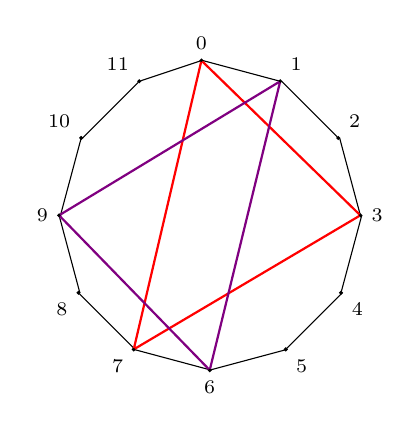
\begin{tikzpicture}
    \node[
        draw,fill,circle,
        %mininum size=3pt,
        inner sep=0pt,outer sep=0pt,
        label=above:{\scriptsize${0}$}] (A0) {}; 
    \foreach \ang[
        count = \n,
        evaluate = \n as \prev using \n-1,
        evaluate = \ang as \labelang using {mod(450-30*\n,360)},
        %evaluate = \ang as \edgeang using {mod(450-30*\n,360)},
    ]in {330,300,...,60,30}{%
        \node[
            draw,fill,circle,
            %mininum size=3pt,
            inner sep=0pt,outer sep=0pt,
            label=\labelang:{\scriptsize$ {\n}$}
        ] (A\n) [angle={\ang+15}{of A\prev}] {} edge (A\prev);
    }
    \draw (A0) -- (A11);

    \draw[thick,red] (A0) -- (A3) -- (A7) -- (A0);
    \draw[thick,violet] (A6) -- (A9) -- (A1) -- (A6);

\end{tikzpicture}

\end{document}
